\subsection{Implicit Methods for Initial-Boundary Problems}

\begin{frame}{Implicit Methods for Initial-Boundary Problems}

\rightline{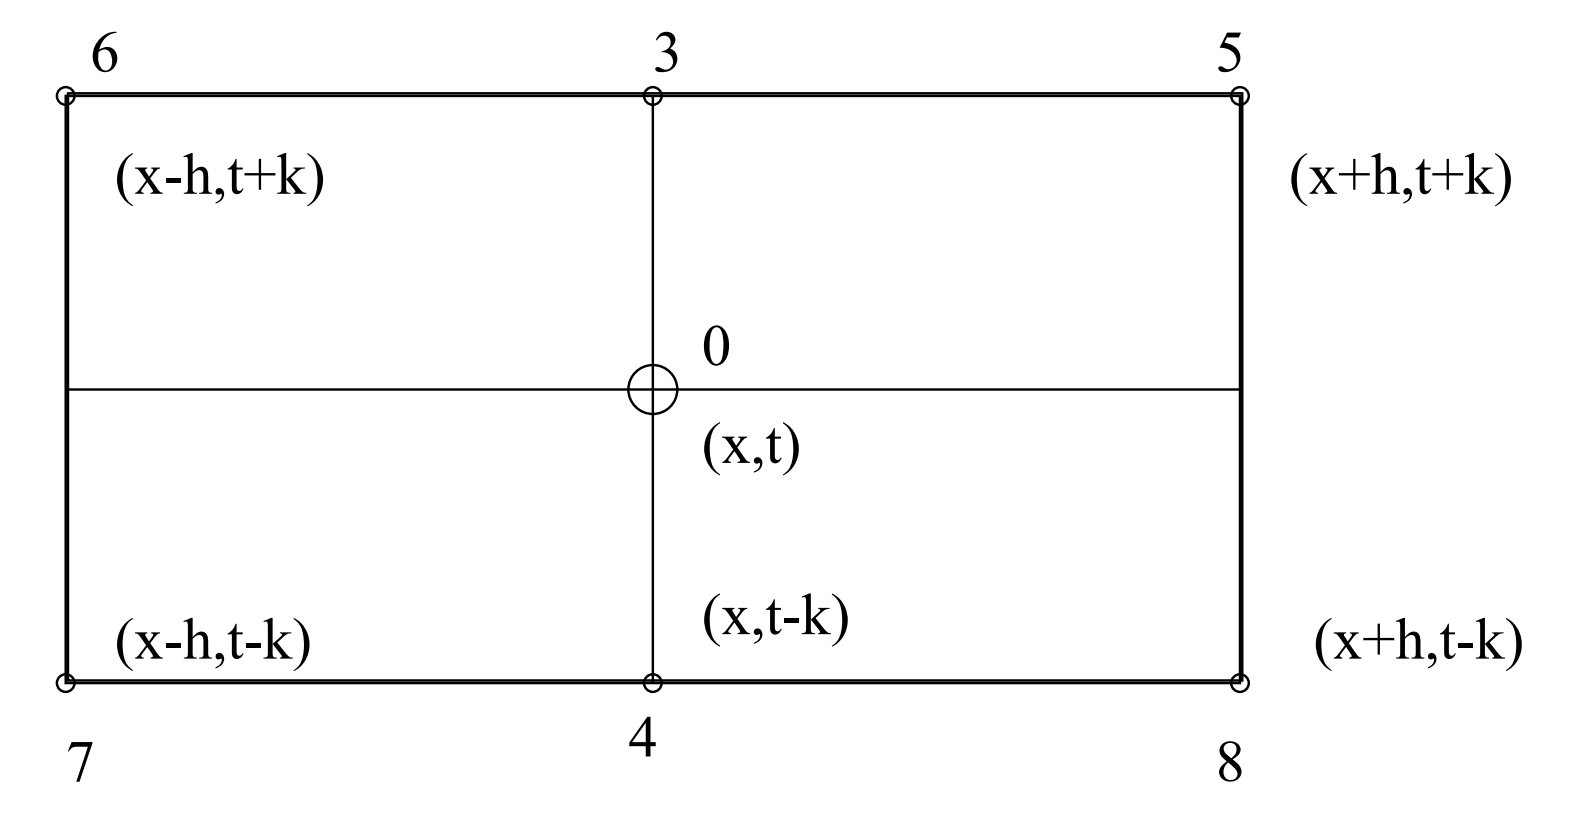
\includegraphics[height = 0.62 \textheight]{img/23/implicit_for_initial}}
\end{frame}


\begin{frame}
\begin{multline}U_{xx}(x,t) = \frac{1}{2} \left [ \frac{u(x-h,t+k) -2u(x,t+k)+u(x+h,t+k)}{h^2} \right. \\
 \left.+ \frac{u(x-h,t-k)-2u(x,t-k)+u(x+h,t-k)}{h^2}\right ]\end{multline}
\vspace{2mm}
\begin{equation}u_{tt}(x,t) =  \frac{u(x,t+k)-2u(x,t)+u(x,t-k)}{k^2} \end{equation}
\vspace{2mm}
\begin{equation}u_6 -2 \left (1 + \frac{h^2}{k^2} \right )u_2 + u_5 = -u_7 +2\left (1 + \frac{h^2}{k^2}\right ) u_4 - u_8 - 4 \frac{h^4}{k^4}u_0\end{equation}
\vspace{2mm}
\center{$\rightarrow$ układ równań z macierzą trójdiagonalną}
\end{frame}


\subsection{Mildy Nonlinear Problems}
\begin{frame}{Mildy Nonlinear Problems}
\begin{block}{}
\begin{equation}u_{xx} - u_{tt} = f(x,t,u) \end{equation}
\end{block}
W metodzie jawnej: \\

\begin{equation} \begin{split} \frac{u(x-h,t) - 2 u(x,t) + u(x_h,t)}{h^2} - \frac{u(x,t+k) - 2u(x,t) + u(x,t-k)}{k^2} \\
= f(x,t,u(x,t)) \end{split} \end{equation}
\end{frame}

\begin{frame}
\textbf{The Cauchy Problem -- D'Alambert formula}
 \centerline{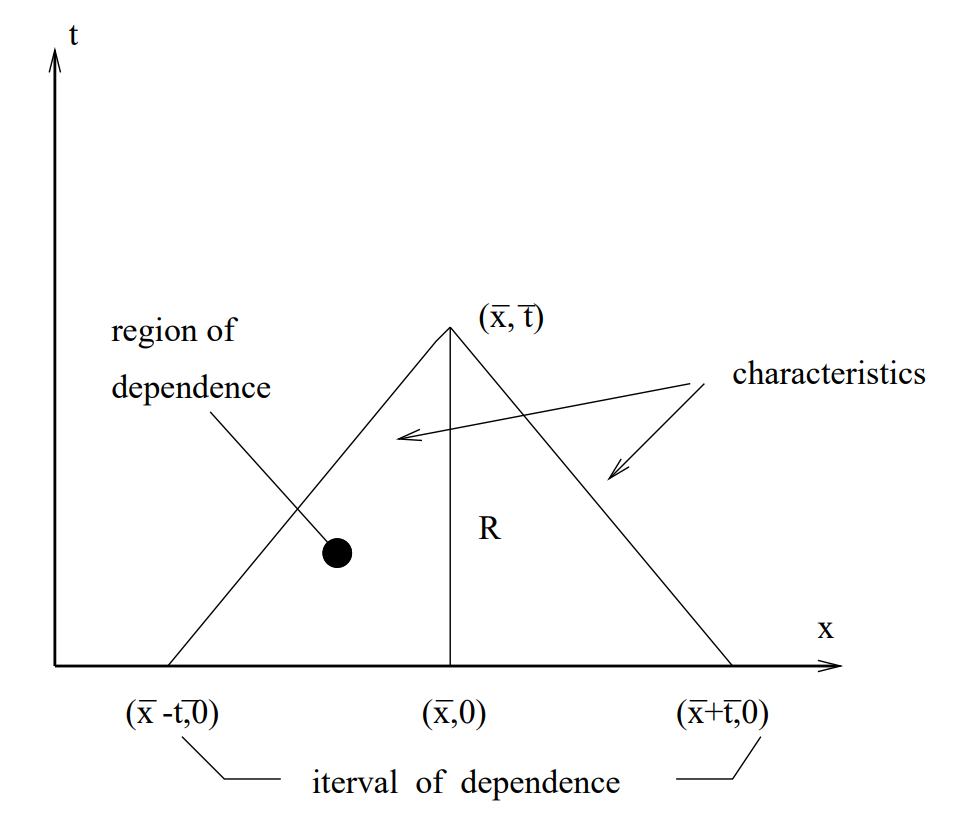
\includegraphics[height = 0.8 \textheight]{img/23/mildy_nonlinear}}
\vspace{5mm}

\end{frame}

\begin{frame}
\begin{equation}u(\overrightarrow{x},\overrightarrow{t}) = \frac{1}{2}\cdot \left [f_1(\overrightarrow{x}+\overrightarrow{t})+f_1(\overrightarrow{x} -\overrightarrow{t}) +\int_{\overrightarrow{x}-\overrightarrow{t}}^{\overrightarrow{x}+\overrightarrow{t}} f_2(r)dr
\right ] \end{equation}
$u(\overrightarrow{x},\overrightarrow{t})$ jest w sposób kompletny określone przez $f_1, f_2$ \\
dla $x \in [(\overrightarrow{x}-\overrightarrow{t},0),(\overrightarrow{x}+\overrightarrow{t},0)]$

charakterystyki:
\begin{equation} t - \overrightarrow{t} = x - \overrightarrow{x}   \quad t - \overrightarrow{t} = -x - \overrightarrow{x}\end{equation}
\vspace{1mm}
Gdy warunek początkowy zadany dla $0 \le x \le a$ wtedy rozwiązanie tylko dla obszaru zależności
 \centerline{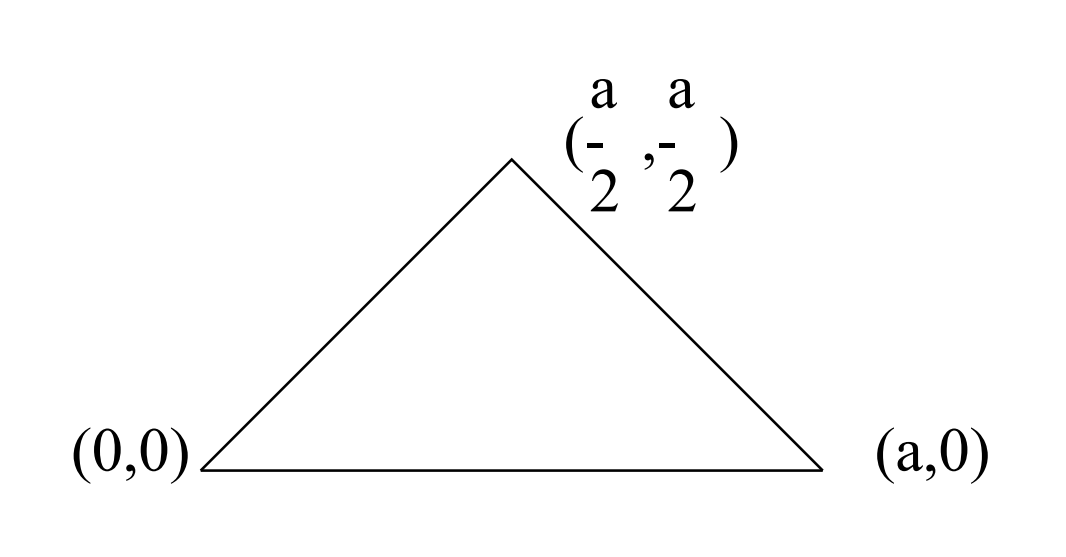
\includegraphics[height = 0.4 \textheight]{img/23/mildy_nonlinear2}}
\end{frame}
